\input{chapter-header.tex}

% ===========================================================================
\chapter{\VTT: Virtualized Application Runtimes}
\chaplabel{vtt}
\minitoc
% ===========================================================================
\introduction
% ===========================================================================

This chapter presents the model of our Virtualization Application Runtime infrastructure, namely \VTT~(cf. Section \ref{sec:virtualization_overview}). In \VTT, an application runtime is virtualized by residing inside a controlled space, namely an \emph{object space}, that encapsulates the access to it. A first-class representation of this object space provides a high-level API to easily query and manipulate the application runtime~(cf. Section \ref{sec:object_space}). The client of an object space is a \emph{runtime hypervisor}~(cf. Section\ref{sec:hypervisor}).

\begin{figure}[htb]
\begin{center}
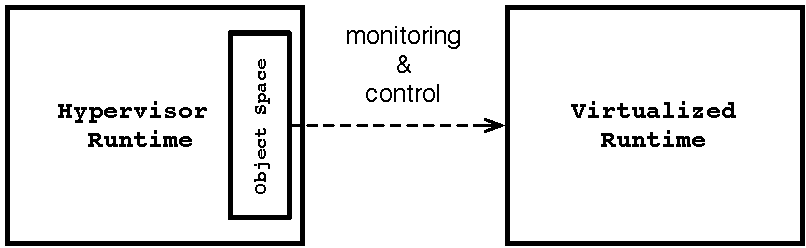
\includegraphics[width=.7\linewidth]{virtualization_introduction}
\caption{\textbf{Virtualization concepts in \Vtt.}\label{fig:virtualization_introduction}}
\end{center}
\end{figure}

The runtime hypervisor runs in the same process than the virtualized runtime to monitor and manipulate it directly. However, the runtime hypervisor does not share the same application runtime than the virtualized runtime it supervises \ie basic objects, classes and \VM structures are not shared between the runtime hypervisor and the virtualized runtime. Instead, both the virtualized and hypervisor runtimes contain their own copies of those elements. This no sharing strategy pursues to allow the hypervisor to change any part of the virtualized runtime without affecting itself as it happens in reflective architectures~(cf. Figure \ref{fig:virtualization_introduction}).

A first class runtime hypervisor manipulates the virtualized runtime through a first-class object space object. This hypervisor can also perform cross-runtime message-sends by injecting processes, as the direct message-send \VM mechanism would fail the method lookup~(Section \ref{sec:isolation}).
Finally, a more granular control can be made through virtual execution. For this, a virtual code interpreter provides full intercession power over the execution of the virtualized application for usages such as tracing or debugging~(Section \ref{sec:interpretation}).

This chapter focuses on the model of our solution and presents its core ideas. The following \chapref{prototype} will present the particular implementation details of our prototype implementation of \Vtt on Pharo.

%On one side, this means that the hypervisor can freely manipulate the virtualized language runtime without affecting itself. On the other side, this no-sharing strategy poses an extra effort in communication~(cf. Section \emph{sec:isolation}) mainly in object marshaling.

%A language hypervisor is a first-class object in \VTT, meaning that we can easily modify it and replace it by another object. Additionally, a simulation mode allows a fully-managed execution mode.

%We do not require any changes in existing applications to import them inside an object space. We introduce minimal modifications at the \VM level to ensure their control and manipulation is transparent. Regarding execution, an object space provides with different means for controlling the execution of the language runtime it owns~(cf. Section \ref{sec:execution}). It can safely start, pause and resume its execution, create new threads or finalize existing ones.  


\section{\Vtt Architecture} \label{sec:virtualization_overview}

\Vtt presents an architecture where multiple application runtimes can co-exist on the same process independently from each other. They do not share any \VM or language state \ie each one has its own interpreter, stack, classes and objects. In this setting, a virtualized application runtime is an application runtime that is monitored by another application runtime. The application runtime that takes the role of controlling the virtualized runtime is the hypervisor runtime. The hypervisor runtime is a full-fledged application runtime, providing us with the expression power and abstractions of a high-level language to express our runtime hypervisor. A first-class object space object represents the virtualized runtime and provides operations for its manipulation. A first-class runtime hypervisor object uses the object space and implements a particular manipulation on it \eg runtime update, failure detection, browsing and debugging. Figure \ref{fig:objectSpaceOverview_architecture} provides an overview of the \Vtt's architecture.

\begin{figure}[htb]
\begin{center}
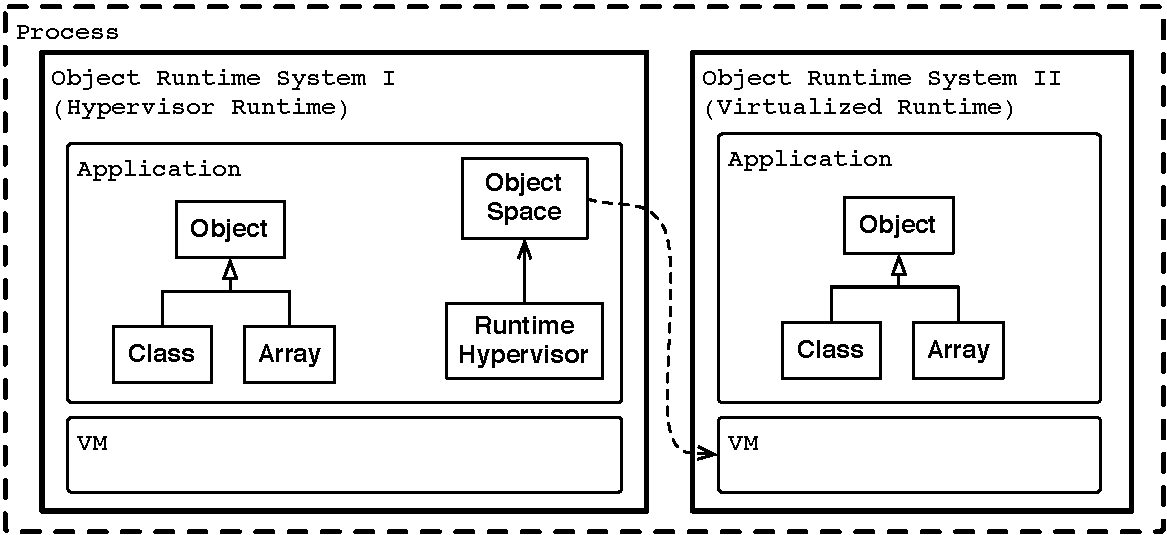
\includegraphics[width=1\linewidth]{object_space_overview3}
\caption{\textbf{\VTT Overview.} A runtime hypervisor in the runtime I (left) manipulates the runtime II (right) through an object space.\label{fig:objectSpaceOverview_architecture}}
\end{center}
\end{figure}

An object space manipulates the virtualized runtime directly, changing the target's application runtime state and manipulating the \VM-language interface. All modifications are applied from the outside of the target virtualized runtime, in contrast with reflective architectures where such changes are applied from the same application runtime under modification. Doing so provides \Vtt with the following properties:

\begin{description}
\item[Transparency.] Our solution does not require any changes in the applications residing inside the virtualized runtime. Thus, we can virtualize existing application runtimes without modifying them \ie \Vtt does not require virtualized applications to include particular libraries, use particular interfaces nor change their execution model.

\item[Application independence.] Our solution does not depend on the particular application inside the virtualized runtime. Different runtime hypervisors can be written for different use cases, including application specific and general ones. The limitation of this approach is, however, its dependance on the execution model imposed by the \VM.
\end{description}

\section{Object Spaces: First-class Application Runtimes} \label{sec:object_space}

An object space is a first-class representation of an object oriented application runtime, meant for its manipulation and control. An object space encapsulates an application runtime and provides with a clear and explicit interface to manipulate it. This interface is split in two different kind of objects: an \ct{objectSpace} object provides general operations on the virtualized runtime while mirror objects~\cite{Brac04b} provide operations to manipulate individual objects that reside inside it~(Figure \ref{fig:objectSpaceMirrors}). Specific mirrors, such as the \ct{ClassMirror}, manipulate elements with a different object-format or runtime representation to enforce their internal representation.

\begin{figure}[htb]
\begin{center}
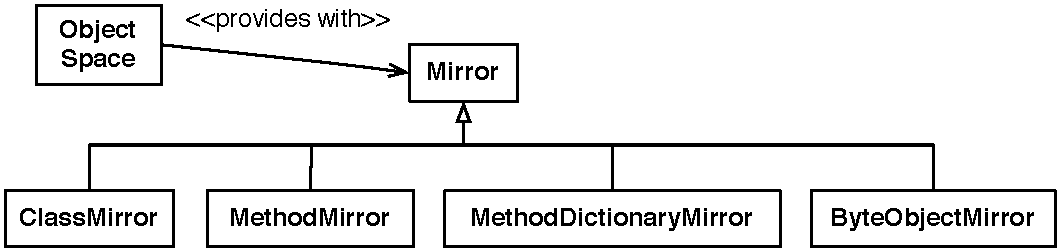
\includegraphics[width=.9\linewidth]{object_space_mirrors}
\caption{\textbf{Mirrors in Object Spaces.} An object space is the main entry point for runtime manipulation. An object space provides with mirrors to modify particular runtime elements. \label{fig:objectSpaceMirrors}}
\end{center}
\end{figure}

These objects make explicit through the operations they expose two important parts of a \VM-language interface, explained in detail in the following subsections. First, The \VM setup interface exposes the elements of the language that should be initialized so it can run a program. Second, the runtime manipulation interface exposes operations that take part at runtime to manipulate runtime structures such as objects, classes, threads, the execution stack.

\subsection{\VM Setup Interface}

The \VM setup is the configuration the \VM needs to run.
For example, a \VM may need the boolean objects \ct{true} and \ct{false} to push them as the result of a boolean operation at runtime.
This configuration is usually done only during the language runtime initialization, before execution of a program, as the \VM cannot easily anticipate the usage of such elements in a program from beforehand.
The \VM setup interface allows us to configure the following kind of elements:

\begin{description}
\item[Well-known objects of the language.] Objects such as \ct{nil}, \ct{true} or \ct{false} are needed at runtime for different purposes. For example, the garbage collection needs \ct{nil} at runtime to update weak references. Other particular objects may be held by the \VM as prototypes to speed-up instantiation time of commonly used objects.

\begin{code}
ObjectSpace {
    mirror getNil();
    mirror getTrue();
    mirror getFalse();

    void setNil(mirror aNilObject);
    void setTrue(mirror aTrueObject);
    void setFalse(mirror aFalseObject);
}
\end{code}

\item[Special classes.] Special classes are those needed by the \VM at runtime. They are needed to perform safety checks, create instances or handle special cases such as immediate objects. For example, when mutating a \ct{String} object the Pharo \VM checks that the introduced object is a \ct{Character} object, to avoid putting the \ct{String} into an invalid state. Also, the \VM requires references to those classes that it instantiates directly~(instead of being created through the \ct{new} message in program). For example, the Pharo \VM instantiates a \ct{BlockClosure} object when it founds the bytecodes that correspond a block expression at runtime. Finally, immediate objects are objects that are encoded inside an object reference instead of occupying a place inside the heap. Immediate objects do not include a reference to their class and therefore the \VM needs to know how to map each particular reference encoding to its corresponding class to perform the method-lookup. 

\begin{code}
ObjectSpace {
    void setArrayClass(classMirror anArrayClass);
    void setBlockClass(classMirror aBlockClass);
}
\end{code}

\item[Special messages.] Special messages are callbacks that the \VM will invoke into the application to notify particular events. The probably most known of such messages is Smalltalk's \ct{doesNotUnderstand}~(the equivalent to \eg Ruby's \ct{methodMissing}). When the \VM does not find a method matching a message-send, it will send a \ct{doesNotUnderstand} message to the receiver object and let the user program decide what to do in such a case.

\begin{code}
ObjectSpace {
    void setDoesNotUnderstandSelector(mirror aSelector);
}
\end{code}

\end{description}

This \VM setup interface avoids to hardcode particular knowledge of a language inside the \VM. This gives us the possibility to easily change particular language internals such as renaming special messages or changing the class hierarchy of special classes without leaving the runtime in an inconsistent state. Being radical, we could think on porting another language to this VM, as long as they share similar execution semantics \ie the \VM execution model is compatible with the given language and we configure this interface accordingly.


%In our particular implementation the list of classes exposed through this interface are those of literal objects and those related with the internal \VM execution model. For the sake of completeness the list of classes is the following: \ct{Array}, \ct{Association}, \ct{BlockClosure}, \ct{ByteArray}, \ct{ByteString}, \ct{ByteSymbol}, \ct{Character}, \ct{Context}, \ct{Float}, \ct{SmallInteger}, \ct{LargePositiveInteger}, \ct{LargeNegativeInteger}, \ct{Message}, \ct{CompiledMethod}, \ct{MethodDictionary}, \ct{Semaphore}, \ct{WeakFinalizationList}.

\subsection{Runtime Manipulation Interface} 
The runtime manipulation interface includes operations to monitor and modify the application runtime during execution. This interface provides access to the application runtime internal elements and encapsulate the implementation details behind them~(\ie the object-format imposed by the \VM). This interface provides the following kind of operations:

\begin{description}
\item[Runtime Global Access.] An object space offers operations to query and modify the global state of the runtime. For example, it provides access to the loaded classes or the running threads/processes. It exposes as well operations to install new and remove existing ones.

\begin{code}
ObjectSpace {
    "Classes"
    mirror createClass(String name, int formatOfInstances);
    List<mirror> getClasses();
    mirror getClass(String name);
    void removeClass(String name);
    ...

    "Threads"
    List<mirror> getThreads();
    List<mirror> instalThread(threadMirror thread);
    ...
}
\end{code}

\item[Runtime Object Access.] Mirrors~\cite{Brac04b} expose the operations to query or alter a particular object or element in the runtime. Different kind of mirrors honor the object-format of the different type of objects we can manipulate. For example, we expose specific mirrors for normal objects, classes, methods, activation records or processes. Notice that these mirrors are low-level mirrors as they expose operations to mutate and access objects in their \VM representation. Additionally, through mirrors we can execute \VM primitives on objects, providing the correct primitive ID~(an integer or native function pointer, depending on the implementation) and the corresponding arguments. These primitives are operations that the \VM exposes normally to the language.

\begin{code}
Mirror {
    "Class access"
    classMirror getClass();
    void setClass(classMirror aClass);

    "Field Access"
    mirror getInstVar(String varName);
    void setInstVar(String varName, mirror anObject);
    
    "Primitive execution"
    mirror executePrimitive(primitiveID id, mirror receiver, Array args);
}
\end{code}

\begin{code}
ClassMirror {
    "Instantiation"
    mirror instantiate();
    mirror instantiate(int aSize);

    "Method manipulation"    
    void compileMethod(String sourceCode);
    void removeMethod(String selector);
}
\end{code}

\end{description}

% ===========================================================================

\section{First-Class Runtime Hypervisors}\label{sec:hypervisor}

The client of an object space is a \emph{runtime hypervisor}. A runtime hypervisor is first-class entity that implements a particular monitoring/modification strategy. A runtime hypervisor monitors an object space by splitting the execution in cycles. These cycles are delimited by a time window and finished in safe suspension points~(Figure \ref{fig:execution_cycle})\ie a safe suspension point is a moment in execution where suspending a thread will not leave it in an inconsistent state. For example, in our \Vtt prototype written for the Pharo language, safe suspension points are the activation of message sends and bytecode backjumps. During each execution cycle, the virtualized runtime runs unmanaged using the full \VM's capacity. When the cycle finishes because the execution completed a time window and found a suspension point, the control is returned to the runtime hypervisor. Then, the runtime hypervisor applies its corresponding action and resumes the execution of the virtualized runtime from the last suspension point.

\begin{figure}[ht]
\center
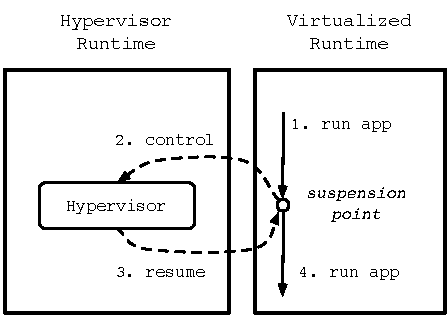
\includegraphics[width=.6\linewidth]{execution_cycle}
\caption{\textbf{Execution Cycle.} \label{fig:execution_cycle}}
\end{figure}

To allow cycle execution, we extended the \ct{objectSpace} interface to execute during a cycle of time. An \Vtt implementation should additionally include support for suspension points. This operation will awake the virtualized runtime processes and execute them for a time window. Once the time window is finished, it will be suspended in the next suspension point and the control will return to the runtime hypervisor.

\begin{code}
ObjectSpace {
    void runCycle();
}
\end{code}

%Our implementation presents an execution cycle of 200ms that allows us to have fine grained control while the virtualized application has still place to run. We use as suspension points backjumps found in the executed bytecode and message sends. In such a way, we ensure that the execution stack is in a consistent state after it is interrupted.

Then, our runtime hypervisor class hierarchy presents four basic methods. First, the \ct{run} template method implements the basics of the hypervision cycle: it resumes the execution of the virtualized runtime inside a loop. Two methods~(\ct{before} and \ct{after}) provide hooks for the specific hypervisor implementations. Figure \ref{fig:hypervisors} shows a class hierarchy example and code with two sketched runtime hypervisors. A \ct{NullHypervisor} allows the virtualized runtime to run without any intervention. The \ct{UpdateHypervisor} instead checks the existence of a file with updates on every cycle.

\begin{code}
Hypervisor >> run
    [ true ] whileTrue: [
        self before.
        self basicRun.
        self after.
    ]

Hypervisor >> basicRun
    objectSpace runCycle.

NullHypervisor >> before
    "Nothing"

NullHypervisor >> after
    "Nothing"

UpdateHypervisor >> before
    self checkForUpdate.

UpdateHypervisor >> checkForUpdate
    "We check if a given file exists"
    'update.txt' asFile exists ifTrue: [ ...
    ...
\end{code}

\begin{figure}[ht]
\center
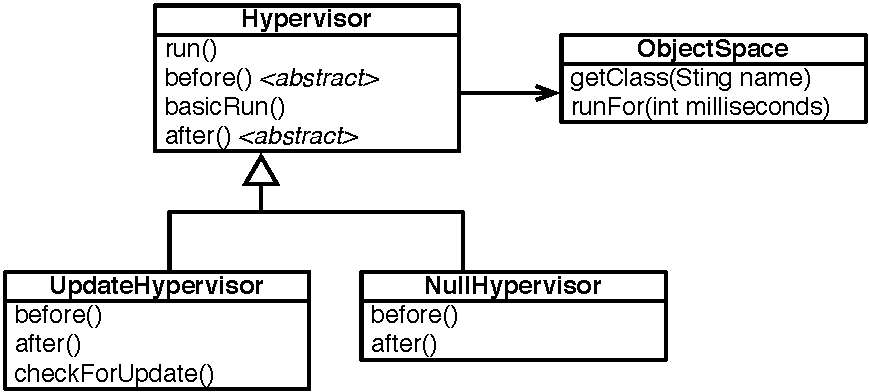
\includegraphics[width=.9\linewidth]{hypervisors}
\caption{\textbf{Example Runtime Hypervisors Class Hierarchy.} A \ct{NullHypervisor} does nothing while the \ct{UpdateHypervisor checks for updates before every cycle execution}.\label{fig:hypervisors}}
\end{figure}

\section{Cross-Runtime Communication} \label{sec:communication}\label{sec:isolation}

A runtime hypervisor may require to apply some operation in a virtualized runtime that would be more difficult through direct object manipulation with mirrors. Let's take as an example a virtualized application that uses a particular logging library. In the context of that application, disabling logging would mean to execute the following statement:

\begin{code}
Logger disable.
\end{code}

And the code invoked should be:

\begin{code}
Logger class>>disable
	self uniqueInstance disable
	
Logger>>disable
	enabled := false
\end{code}

However, doing the same through our abstract layer of mirrors presents the following drawbacks (a) to replicate the behavior of the \ct{disable} method inside the hypervisor and (b) to couple it to the internals of such a logging library. 

\begin{code}
OurHypervisor>>disableLogging
	logger := objectSpace getClass: #Logger.

	"the logger is a singleton"
	"in a class variable named uniqueInstance"
	loggerInstance := logger classVariablesAt: #UniqueInstance.

	"The enabled instance variable is the first"
	loggerInstange instanceVariableAt: 1 put: false.
\end{code}

Thus, a runtime hypervisor may benefit from the execution of an arbitrary expression or statement within the scope of the virtualized runtime. For example, enabling or disabling a logger from the virtualized application can be easily achieved through executing the following statement in the runtime hypervisor instead of manually modifying the state of the logger objects:

\begin{code}
objectSpace execute: [ Logger disable ].
\end{code}

To achieve this kind of communication, we observe the following challenges in using a plain \VM's message-send mechanism with our no sharing strategy.

\begin{description}

\item[Cross-Runtime Method-Lookup.]A \emph{cross-runtime message-send}~(from the hypervisor to the virtualized runtimes) cannot be simply achieved by the usual message-send mechanism. The usual message-send mechanism looks up in the receiver's class hierarchy a method with an \emph{object identical} method signature. However, our not-sharing strategy prevents the normal method-lookup work on a \emph{cross-runtime message-send} as symbols and classes are not shared between the different runtimes. In such a case, the method-lookup mechanism fails because the elements of a message signature and the method signature we target are indeed \emph{equals but not identical}~(Figure \ref{fig:cross_runtime_lookup}).

\begin{figure}[ht]
\center
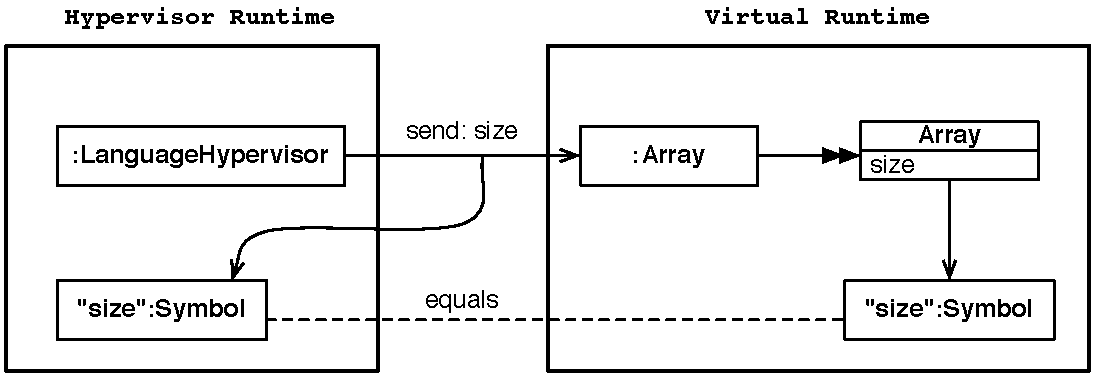
\includegraphics[width=.9\linewidth]{cross_runtime_lookup}
\caption{\textbf{Failing Cross-Runtime Method Lookup.} The runtime hypervisor sends the \ct{size} message to an array in the virtualized runtime. This message-send signature is the hypervisor runtime's \ct{size} symbol. The \ct{size} method exists but its signature has a different \ct{size} symbol. Both symbols are equals but not identical, and thus the lookup fails.\label{fig:cross_runtime_lookup}}
\end{figure}

\item[Exceptions and Stack.] A cross-runtime method-lookup succeeds if we modify the runtime hypervisor message-send to contain the right symbol from the virtualized runtime. In such case, the execution stack contains a mixture of activations that belong to the hypervisor and virtualized runtimes. This poses a problem under the presence of techniques that traverse the execution stack indiscriminately, such as the exceptions or stack manipulation techniques such as Smalltalk's \ct{thisContext} special variable. The presence of such elements may leak object references from a runtime to another, leaving them in inconsistent state~(Figure \ref{fig:mixed_stack}) \gp{cite some paper like j kernel on exceptions leaking references}.

\begin{figure}[ht]
\center
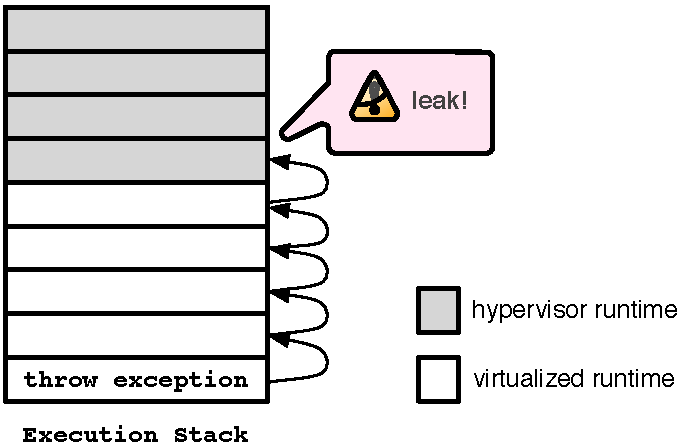
\includegraphics[width=.6\linewidth]{mixed_stack}
\caption{\textbf{Reference Leaks in a Mixed Stack on Exception.} When mixing the execution stack between the virtualized and hypervisor runtimes, an exception may traverse the stack and have access to a reference from a different runtime.\label{fig:mixed_stack}}
\end{figure}

\end{description}

To overcome these problems we base the cross-runtime communication on \emph{process injection}. We create a new process/thread inside the virtualized runtime containing the expression to execute. The new process is installed in the virtualized runtime and executed in cycles until it is finished. Once finished we can access the result of the expression through a mirror. The objects that conform the message-send signature and other literals~(\eg strings, numbers) are translated from their representation in the hypervisor runtime to their corresponding representation in the virtualized runtime. Global object references such as classes are mapped to their corresponding references in the virtualized runtime. Non-global non-literal objects can be specified explicitly as an argument:

\begin{code}
objectSpace
	execute: [ :aLogger | aLogger disable ]
	with: aLoggerInstanceMirror.
\end{code}

This solution for cross-runtime communication solves both problems observed before. In a first place, it prevents the method-lookup failure by translating the objects part of the method signature. Second, the new process executes in its own stack ensuring none of the objects from the hypervisor are leaked to the virtualized runtime.

\section{Virtual Execution through Interpretation} \label{sec:interpretation}

\Vtt allows a \emph{virtual execution} mode through interpretation. Virtual execution takes place by doing code interpretation of either abstract syntax trees~(ASTs) or bytecode. In \Vtt a virtual code interpreter is a first-class entity that interprets code inside a virtualized runtime and has full control on the interpreted code. The virtual interpreter is useful in cases where the virtualized runtime is in an incoherent or buggy state and it cannot execute code by itself. In those cases, the virtual interpreter can be used to fix the problem in the virtualized runtime before it can continue its own execution. For example, we can use the virtual code interpreter to replace a broken method in the basic class hierarchy:

\begin{code}
"newMethod is a method that fixes the bug"
interpreter := VirtualCodeInterpreter newOn: anObjectSpace.
interpreter
	execute: 'Object methodDictionary at: #brokenSelector put: newMethod'
	with: newMethod.
\end{code}

The virtual code interpreter has three main points of communication with an object space:

\begin{description}
\item[Instance Variable Access.] Accessing or writing an object's instance variable is mapped by the code interpreter to a field access or write in the mirror representing the receiver object.

\begin{code}
VirtualCodeInterpreter >> readInstanceVariableNumber: index
    ^ self receiver instanceVariableAtIndex: index
    
VirtualCodeInterpreter >> writeInstanceVariableNumber: index with: aMirror
    ^ self receiver instanceVariableAtIndex: index put: aMirror
\end{code}

\item[Method Lookup.] On a message-send, the virtual code interpreter performs the method lookup by inspecting the class hierarchy of the receiver object. The receiver object state is exposed to the interpreter by a mirror. Following, we illustrate this with a simplified method lookup:

\begin{code}
VirtualCodeInterpreter >> lookupSelector: selector
    | classToLookup |
    "classToLookup is a class mirror"
    classToLookup := self receiver getClass.
    [ classToLookup isNotNil ] whileTrue: [
        (self class: classToLookup hasSelector: selector)
        	    ifTrue: [ ^ classToLookup ].
	classToLookup := classToLookup superclass.
    ]
\end{code}

\item[Primitive Execution.] In the leaves of the execution, message-sends invoke the language primitives. These language primitives are executed through the object space interface.

\begin{code}
VirtualCodeInterpreter >> invokePrimitiveMethod: aMethod
    ^ self objectSpace
         executePrimitive: aMethod primitive
         receiver: self receiver
         arguments: self arguments
\end{code}

\end{description}

Being a first-class entity, we can specialize the code interpreter to instrument code execution in order to override normal behavior or trace the execution. We can for example trace all instance variable writes by overwriting one of the methods above.

\begin{code}
TracingCodeInterpreter >> writeInstanceVariableNumber: index with: aMirror
    | result |
    result := super writeInstanceVariableNumber: index with: aMirror.
    !\emph{self logWriteIn: self receiver atIndex: index with: aMirror.}!
    ^ result
\end{code}

% =============================================================================
\section{Conclusion and Summary}

\Vtt presents an architecture where several application runtimes can share the same process. A virtualized application runtime is subject of monitoring and manipulation from another application runtime, namely the hypervisor runtime. The hypervisor runtime contains a first class representation of the virtualized runtime, an object space. The object space exposes a clear interface to safely access and modify an application runtime. This interface includes operations to configure the virtualized application runtime and operations to modify particular objects from it. The latter is encapsulated in mirror objects.

The execution of the virtualized runtime is organized in cycles. In between cycles, a first-class runtime hypervisor can perform an operation and then resume the virtualized runtime's execution. We ensure that the state of the virtualized runtime keeps its coherence by only suspending it in safe suspension points.

Besides the direct manipulation through mirrors, a runtime hypervisor can perform cross-runtime message-sends for a richer communication using process injection. Process injection prevents failures in the method lookup and avoids stack traversing techniques such as exception to leak cross-runtime references. Additionally, a virtual code interpreter allows us to execute code on the virtualized runtime with full intercession. A virtual code interpreter is a first class entity, allowing us to easily specialize and change it.

In following chapters we will show how this infrastructure supports the evolution of a programming application runtime in two different scenarios. First, the recreation of a application runtime using an explicit bootstrap process. Second, an application tailoring technique that specializes an application runtime to contain only elements that are used during runtime.

\input{chapter-footer.tex}